%=================================================
\documentclass[12pt]{article}
\usepackage[left=3cm, right=2cm, top=3cm,bottom=2cm]{geometry}
\usepackage{fancyhdr}
\usepackage{listings}
\usepackage{float}
\usepackage[utf8]{inputenc}
\usepackage[brazil]{babel}
\usepackage{graphicx}
\usepackage{latexsym,amssymb,amsmath,amsfonts}
\usepackage{url}
\usepackage{indentfirst}
\usepackage{enumerate}
\usepackage{setspace}
\usepackage{placeins}
\usepackage{listings}
%\usepackage{minted}
 \usepackage{multirow}
\usepackage{subfigure}
\usepackage{enumitem}
\usepackage{subfigure}
\usepackage{wrapfig}
\usepackage{helvet}
\usepackage{epsfig}
%\usepackage{graphicx}
\usepackage{times}
\usepackage{arydshln}
\usepackage{subfigure}
\usepackage{amsmath,amssymb,amsthm}
\usepackage{graphicx}
\usepackage{lastpage}
\usepackage{multirow}
\usepackage{comment}
\usepackage[hidelinks]{hyperref}
%=================================================

\title{Processamento de Imagens}
\author{Paulo César Moraes de Menezes}
\date{\today}

\begin{document}

\maketitle

\newpage

\tableofcontents % Adiciona o sumário

\newpage

\section{Algumas informações iniciais sobre o documento}

Este documento terá todo o meu estudo direcionado ao tema de Processamento Digital de Imagens, a ideia é adicionar informações que foram
adquiridas tanto na disciplina Processamento de Imagens (DCE536) quanto em outras fontes de conhecimento.A ideia é que este documento seja
uma espécie de guia para o meu estudo, e que possa ser útil para outras pessoas que estejam interessadas no tema.
Além disso dedico o meu estudo para aprofundar o meu conhecimento em Inteligência Artificial, que é a área que pretendo seguir na minha
carreira profissional.

% Seu conteúdo aqui
\section{Créditos}

Algumas das informações presentes nesse documento foram extraídas do contéudo fornecido pelo professor Luiz Eduardo da Universidade Federal de
Alfenas.Quero agradecer a ele por compartilhar seu conhecimento na área.Além disso, algumas outras informações serão extraídas de fontes
externas, que serão devidamente referenciadas.

\section{Introdução}



\subsection{O que é Processamento Digital de Imagens?}

Uma imagem pode ser definida como uma função de duas dimensões $f(x,y)$, onde $x$ e $y$ são coordenadas
espaciais em um plano e a amplitude de $f$ em qualquer par de coordenadas $(x,y)$ é chamada de intensidade
ou nível de cinza da imagem naquele ponto.Quando os valores de $x$, $y$ e $f$ são todos finitos e
discretos, chama-se a imagem de imagem digital.No que diz respeito ao campo de processamento digital
de imagens (PDI), o termo refere-se a processar uma imagem por meio de um computador digital.É válido
destacar que uma imagem digital é composta por finitos elementos, cada elemento possuí um valor de
intensidade e posição associado a ele.

Com essas informações em mente, também é válido destacar um dos grandes responsaveis por dar vida a
capacidade de reconhecer imagens: a visão humana.A visão humana é um dos grandes sentidos que o ser
humano possuí, e é também um dos mais complexos.A visão é capaz de capturar e processar
informações visuais de forma extremamente rápida e eficiente.Entretanto, a visão humana não é perfeita, e
também possuí limitações, como por exemplo não ser capaz de enxergar certos comprimentos de onda de
luz, ou ser limitado pelo espectro EM (Eletromagnético) que é capaz de capturar.

Contudo, as máquinas conseguem capturar quase todo o espectro EM, e com isso é possível processar
imagens de forma extremamente eficiente, e é aí que entra o Processamento Digital de Imagens, que é a
área que estuda técnicas e métodos para processar imagens de forma eficiente, e é uma das áreas que
possuí grande importância na área de Inteligência Artificial, pois é uma das áreas que estuda a
capacidade de reconhecer padrões em imagens, que é uma das capacidades que o ser humano possuí.

As máquinas conseguem operar em faixas de frequência que o ser humano não consegue, como por exemplo
raios-x, raios gama, entre outros.

É comum existir um debate do que seria processamento de imagens e visão computacional.Esse debate é
comum, pois as duas áreas possuem muitos pontos em comum, e muitas vezes são utilizadas de forma
intercambiável, entretanto, é válido destacar que as duas áreas possuem diferenças, e que a visão
computacional é uma área que estuda como as máquinas podem ser capazes de interpretar e entender o
mundo visual, enquanto que o processamento de imagens é uma área que estuda como as imagens podem ser
processadas de forma eficiente.O processamento de imagens concentra-se principalmente em técnicas e algoritmos para manipular e
melhorar imagens digitais.Isso inclui operações como filtragem, realce de borda, remoção de ruído,
entre outros, com o objetivo de melhorar a qualidade ou extrair informações úteis das imagens.


 \subsubsection[Processos de baixo nível]{Processos de baixo nível}
Esses processos são conhecidos também como processos primitivos ou pré-processamento, e são processos
para reduzir ruído, realçar bordas, corrigir desfoque, entre outros.

Um processo de baíxo nível é caracterizado pelo fato de que a sua entrada e saída são imagens, e que
não existe um conhecimento prévio sobre o conteúdo da imagem, ou seja, o processamento é feito de forma
cega, sem saber o que está sendo processado.

 \subsubsection[Processos de médio nível]{Processos de médio nível}

O processo de médio nível envolve técnicas de segmentação, que é o processo de dividir a imagem em
partes, ou seja, é o processo de dividir a imagem em partes que são de interesse, e partes que não são
de interesse.Essa segmentação pode ser feita separando a imagem em regiões ou em objetos.Além disso
esse tipo de processo envolve uma descrição sobre os objetos segmentados de modo a reduzi-los de uma
forma adequada para o processamento computacional e a classificação de objetos individuais.

Além disso uma outra característica desse tipo de processo está no fato de que as entradas são
imagens, mas as saídas são atributos extraídos dessas imagens, como por exemplo, a forma, a cor, a
textura, entre outros.

 \subsubsection[Processos de alto nível]{Processos de alto nível}

Esse tipo de processo envolve dar sentido ao conteúdo da imagem, ou seja, envolve a interpretação do
conteúdo da imagem, e é um dos processos mais complexos, e que envolve a utilização de técnicas de
inteligência artificial, como por exemplo, redes neurais, entre outros.

\subsection{As origens do Processamento Digital de Imagens}

Uma das primeiras aparições das imagens digitais foi no jornal industrial no começo dos anos 1920,
na qual foi enviado através de submarinos entre Londres e Nova York, e foi a primeira vez que uma
imagem foi transmitida de forma eletrônica.Esse feito reduziu para horas um trabalho que levava
semanas para ser feito.

\begin{figure}[h]
  \centering
  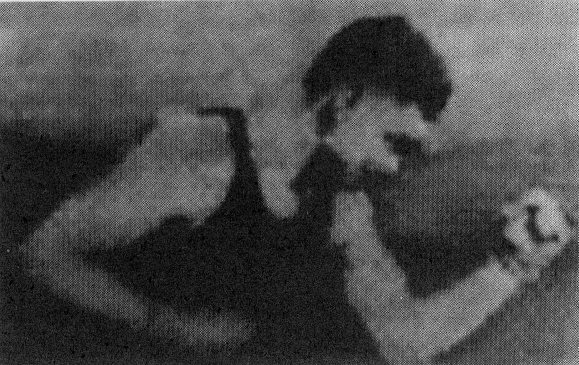
\includegraphics{images/3 2}
  \caption{Imagem digital produzida por fita codificada.}
  \label{fig:exemplo}
\end{figure}

Essas capturas pioneiras tinham capacidade de reconhcer até 5 tons de cinza.Esse valor foi aumentando
até que em 1929 alcançou a incrível marca de 15 tons de cinza.

Um grande fator que limitou o avanço das imagens digitais foi a falta de tecnologia para armazenar
essas imagens, é nítida a relação de dependência entre poder computacional e armazenamento de imagens.

Ao longo do século XX, o PDI foi se desenvolvendo, e foi se tornando uma área de grande importância
para a sociedade, e com a medida que a técnologia computacional evoluia, principalmente durante a
corrida espacial, o PDI foi se tornando uma área de grande importância para a sociedade.


\begin{figure}[h]
  \centering
  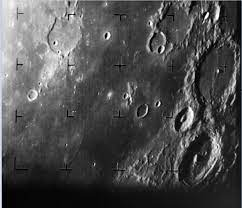
\includegraphics{images/2}
  \caption{Primeira imagem digital da Lua, em 1964.}
  \label{fig:exemplo}
\end{figure}

Além disso, durante a década de 70, o PDI começou a ter aplicações em medicina, e com isso o PDI
começou a ter um grande impacto na sociedade, principalmente com o desenvolvimento de Tomografias
Computadorizadas, que é uma das grandes aplicações do PDI.

\subsection{Aplicações do Processamento Digital de Imagens}

Atualmente praticamente todas as áreas da sociedade possuem aplicações do PDI, e é uma área que
exerce grande influência na sociedade.

\subsubsection{Imagens Raio-Gamma}

A vasta maioria dos usos nesta área é para aplicações de medicina nuclear e observações astronômicas.

A ideia para a medicina nuclear é aplicar isótopos radioativos em um paciente, e com isso é possível
observar o decaimento desses isótopos.Desse modo, é possível coletar imagens do interior do corpo
humano, e com isso é possível diagnosticar doenças.

\begin{figure}[h]
    \centering
    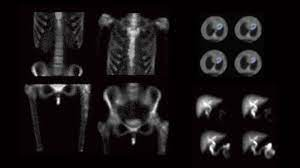
\includegraphics{images/3.jpeg}
    \caption{Gamma Ray Image}
    \label{fig:exemplo}
\end{figure}

\subsubsection{Imagem de Raio-X}

Esta é uma da aplicação mais antigas do PDI, e é uma das aplicações mais conhecidas do PDI.Usada princi
palmente para diagnóstico médico, mas pode ser utilizada em outras áreas, como por exemplo, para
inspeção de bagagens em aeroportos.

\begin{figure}[h]
    \centering
    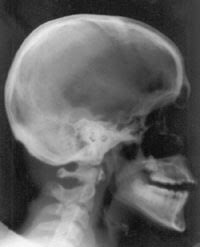
\includegraphics{images/4.jpeg}
    \caption{Raio-X}
    \label{fig:exemplo}
\end{figure}
\newpage

\section{Melhoramento de Imagens}

\subsection{Relacionamento entre Pixels}



\end{document}
